\section{MMArt dataset construction}

\begin{figure*}[ht]
    \centering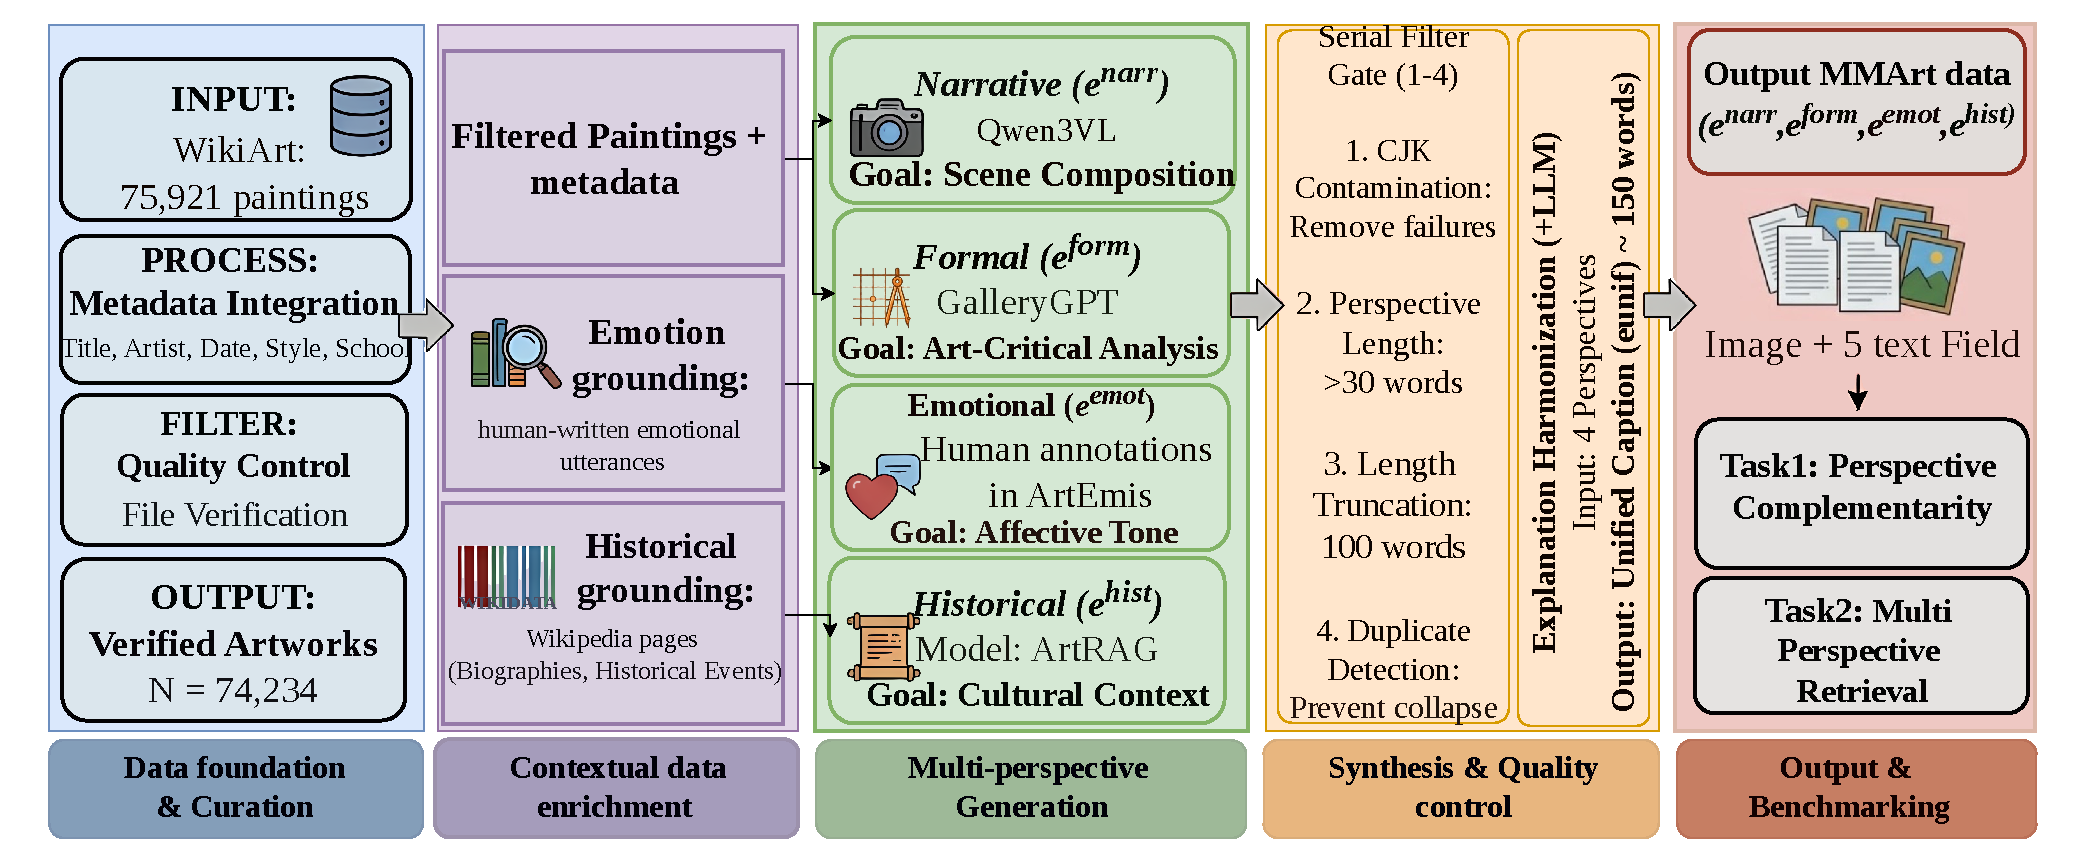
\includegraphics[width=\linewidth]{figures/fig_2_overview.pdf}
    \vspace{-5mm}
    \caption{Overview of the MMArt dataset construction pipeline. Each painting is processed through four specialized vision-language models to produce independently generated perspectives (narrative, formal, emotional, historical), which are then harmonized into a unified caption.}
\label{fig:MMArt_framework}
\end{figure*}

We introduce MMArt, a large-scale multi-perspective dataset grounding visual art understanding in four distinct interpretive dimensions.
This section describes the data foundation, the four-perspective architecture, the model selection and generation pipeline, quality control procedures, and the benchmark task built on the dataset.

\subsection{Data Foundation}

MMArt is built on the WikiArt dataset~\cite{2017omniart}, which covers approximately 75,921 artworks across 20 style categories spanning the 15th through the 21st century.
After filtering to artworks with verified image files on disk and applying quality control, the experiment-ready subset comprises 74,234 paintings from 743 distinct artists, all with complete four-perspective annotations.
Each painting is associated with structured metadata including title, artist name, production date, style classification, and artist school.

\subsection{Four-Perspective Architecture}

Rather than generating a single descriptive caption, MMArt decomposes each artwork's annotation into four independently generated perspectives:

\begin{equation}
P(w) = \{ e^{\text{narr}},\ e^{\text{form}},\ e^{\text{emot}},\ e^{\text{hist}} \},
\end{equation}

where $w$ denotes a painting and each component captures a distinct interpretive dimension.

\paragraph{Narrative and Scene Interpretation ($e^{\text{narr}}$).}
A factual account of the depicted entities, figures, scene composition, and visual elements as they appear in the image.
This perspective answers \textit{what} is shown, without invoking symbolic or historical interpretation.

\paragraph{Formal Visual Analysis ($e^{\text{form}}$).}
An analysis of the painting's compositional structure, including spatial organization, color palette, brushwork, use of light and shadow, and visual rhythm.
This perspective corresponds to the vocabulary of formal art criticism, focusing on \textit{how} the work is constructed.

\paragraph{Emotional Response ($e^{\text{emot}}$).}
An affective characterization of the painting's perceived mood, atmosphere, and psychological tone as registered by a viewer.
This perspective captures the phenomenological dimension of art encounter---\textit{what it feels like} to look at the work.

\paragraph{Historical and Contextual Analysis ($e^{\text{hist}}$).}
An art-historical interpretation situating the work within its cultural context: movement affiliation, iconographic codes, period-specific symbolic meaning, and relevant biographical or historical circumstances.
This perspective answers \textit{why} the work looks and means as it does.

In addition to the four independent perspectives, each painting receives a \textit{unified caption} $e^{\text{unif}}$ produced by harmonizing all four into a single coherent description.
This unified caption serves as a strong single-text baseline in benchmark evaluations.

\subsection{Generation Pipeline}

A central design principle of MMArt is the use of specialized models per perspective, each chosen for its demonstrated strength in the corresponding interpretive task.
Generating all perspectives with a single general-purpose model risks homogenizing the output; using specialized models encourages each perspective to reflect genuine domain fit.

\paragraph{Narrative perspective.}
Narrative captions are generated using Qwen3-VL-8B-Instruct~\cite{bai2025qwen3vltechnicalreport}, a large-scale vision-language model with strong scene understanding.
The 72B scale supports detailed factual description while the model's training on diverse visual corpora reduces systematic bias toward art-specific jargon, keeping the output grounded in observable visual content.

\paragraph{Formal analysis.}
Formal perspectives are generated using specialized GalleryGPT~\cite{MM24GalleryGPT}, a LLaVA-7B model fine-tuned on the PaintingForm dataset specifically for formal art analysis. This specialization ensures that output adheres to the vocabulary and analytical conventions of formal criticism rather than defaulting to general image description.

\paragraph{Emotional response.}
Emotional perspectives are generated using Qwen3-VL-8B-Instruct, conditioned on the painting image together with human-written emotional utterances from the ArtEmis dataset~\cite{achlioptas2021artemis} as few-shot context.
ArtEmis provides on average 5.7 affective utterances per WikiArt painting, grounding the emotional generation in authentic human responses rather than model inference alone.

\paragraph{Historical and contextual analysis.}
Historical perspectives are generated using Qwen3-VL-8B augmented with a Wikidata knowledge graph retrieved via ArtRAG~\cite{ArtRAG_MM2025} in hybrid retrieval mode.
For each artwork, relevant Wikidata snippets covering the artist biography, movement, and historical events are retrieved and injected into the generation context.
This retrieval-augmented approach grounds historical claims in verifiable external knowledge and reduces hallucination of biographical or period-specific facts.

\paragraph{Unified caption.}
Given the four independently generated perspectives $\{e^{\text{narr}}, e^{\text{form}}, e^{\text{emot}}, e^{\text{hist}}\}$, a unified caption $e^{\text{unif}}$ is produced via Qwen3-8B~\cite{bai2025qwen3vltechnicalreport} using a harmonization prompt that synthesizes the four perspectives into a single coherent, non-redundant description of approximately 150 words.
The unified caption preserves interpretive breadth while eliminating cross-perspective repetition, and is designed for downstream tasks such as retrieval and language-model grounding where a holistic single-text representation is preferred.

Formally, the generation of perspective $v$ for painting $w$ with image $I$, metadata $M$, and optional retrieved context $\mathcal{S}$ is:

\begin{equation}
e^{v} = \text{VLM}_v\!\left(I,\ M,\ \mathcal{S},\ \pi_v\right),
\end{equation}

where $\pi_v$ is a perspective-specific prompt template designed to enforce interpretive focus and minimize cross-perspective overlap.

\subsection{Quality Control}

\paragraph{Text quality filtering.}
We apply four automated cleaning steps to the raw generated output.
(i)~\textit{CJK contamination}: perspectives containing Chinese, Japanese, or Korean characters are nulled, as these indicate generation failure on non-Western paintings.
(ii)~\textit{Length filtering}: perspectives under 20 words are nulled as uninformative.
(iii)~\textit{Formal truncation}: $e^{\text{form}}$ exceeding 150 words is truncated at the nearest sentence boundary to remove generation runoff without discarding content.
(iv)~\textit{Duplicate detection}: exact-duplicate $e^{\text{form}}$ values across paintings are nulled, as these indicate model collapse on visually similar inputs.
The full dataset retains all 75,336 paintings with nulls preserved; the experiment-ready subset (`full4') requires all four perspectives to be non-null, yielding 74,234 paintings.

\paragraph{Gold subset evaluation.}
We evaluate perspective quality via an \textit{LLM-as-judge} evaluation reported in Section~\ref{sec:quality}.
Gemma-3-27B~\cite{gemmateam2025gemma3technicalreport}---a vision-language model from a different model family than all generation models---rates all five perspectives on perspective fidelity, factual accuracy, and depth on a stratified 300-painting sample, with both the painting image and WikiArt metadata provided as context.
Using an independent judge from a different model family mitigates self-evaluation bias.

\paragraph{Dataset-level statistics.}
Table~\ref{tab:dataset_stats} summarizes the final dataset statistics, including coverage per perspective and comparison against prior art captioning datasets.


\subsection{Benchmark Task: Perspective Complementarity}

MMArt includes a benchmark for evaluating whether the four perspectives encode genuinely distinct visual information.

\textbf{Question}: Do the four perspectives encode genuinely distinct information, or are they stylistic paraphrases of the same description?

\textbf{Setup}: Given text from one or more perspectives (without the original image), a text-to-image model generates a reconstruction of the original painting.
We evaluate ten perspective conditions: four singles ($e^{\text{narr}}$, $e^{\text{form}}$, $e^{\text{emot}}$, $e^{\text{hist}}$), four leave-one-out triples (each omitting one perspective), the full four-perspective combination, and the unified caption as a holistic baseline.
Each reconstruction is compared to the original across three fidelity dimensions:

\begin{equation}
\mathcal{F}(w, \hat{w}) = \bigl(\delta_{\text{style}},\ \delta_{\text{comp}},\ \delta_{\text{emot}}\bigr),
\end{equation}

where $\delta_{\text{style}}$ is CLIP ViT-L/14 cosine similarity, $\delta_{\text{comp}}$ is DINOv3-Large CLS token cosine similarity capturing spatial structure and composition, and $\delta_{\text{emot}}$ is CLIP zero-shot emotion agreement against nine ArtEmis emotion labels.

\textbf{Hypothesis}: Each perspective recovers a different subset of fidelity dimensions, and reconstruction improves as perspectives are combined.
If perspectives were redundant, adding more would not improve reconstruction fidelity.

\textbf{Scale}: Evaluated on a stratified sample of 1,350 paintings (50 per style $\times$ 27 styles) using two text-to-image models---FLUX.2-Klein-4B~\cite{flux2} and Qwen-Image-2512~\cite{wu2025qwenimage}---to confirm that findings are model-agnostic.

